\documentclass[11pt,a4paper]{article}

\usepackage[margin=2.2cm]{geometry}
\usepackage{graphicx}
\usepackage{booktabs}
\usepackage{tabularx}
\usepackage{float}
\usepackage{caption}
\usepackage{subcaption}
\usepackage{enumitem}
\usepackage{xcolor}
\usepackage[hidelinks]{hyperref}
\usepackage{amsmath}
\usepackage{array}

\graphicspath{{figures/}}
\setlist{nosep, leftmargin=*}
\captionsetup{font=small, labelfont=bf}
\newcommand{\todo}[1]{\textcolor{red}{[#1]}}

\title{\textbf{PakCareer AI}\\[2pt]
\large Data-driven degree guidance for Pakistani college graduates\\[2pt]
\normalsize Deliverable 1: Problem Definition \& Data Foundations (Track A)}
\author{
Kabeer Ahmed Shahzeb (24L-3087) \and Muhammad Hasan Butt (24L-3022) \and Muhammad Moosa Khan Rokhri (24L-3070)\\[4pt]
\small FAST School of Computing, National University of Computer and Emerging Sciences, Lahore
}
\date{October 2026}

\begin{document}
\maketitle

\begin{abstract}
Every year, students finishing intermediate or A-Levels in Pakistan choose a degree that shapes
their whole career, and the choice is very often made by their parents, who default to a small set
of ``safe'' professions. PakCareer AI sorts a student into one of seven degree families
(``houses'') from their interests and personality, and backs the recommendation with
Pakistan-specific labour-market statistics the student can show their family. This report covers
Phase~1 (problem definition) and Phase~2 (data acquisition and preprocessing). We collected five
sources: 145,828 RIASEC interest-test responses (training data), the O*NET 31.0 occupation
database, Pakistan Labour Force Survey indicators from ILOSTAT, World Bank indicators, and
10,999 live Pakistani job postings scraped from Rozee.pk. We also evaluated ten supplementary
Kaggle career datasets and excluded all of them from training: six have random labels, one leaks
the target and three are too small or unlabelled. After cleaning, the modelling table holds
81,256 labelled respondents with 30 engineered, scaled and encoded features. A preliminary
gradient-boosting baseline places the student's actual field among its top three houses
86\% of the time.
\end{abstract}

% ------------------------------------------------------------------
\section{Phase 1: Problem Definition}

\subsection{Problem statement}
In Pakistan the decision of what to study after intermediate (FSc, ICS, ICom, FA) or A-Levels is
frequently taken by the family rather than the student. Medicine and engineering in particular are
treated as default ``respectable'' careers, regardless of whether the student is interested in or
suited to them. The result is students who are unmotivated in their degree, switch fields
mid-way, or graduate into a career they did not want.

Choosing ``any degree'' is also no longer a safe bet. The Labour Force Survey data we collected
(Section~\ref{sec:eda-pk}) shows that in 2025 the unemployment rate among Pakistanis with advanced
(degree-level) education was \textbf{11.1\%}, against \textbf{7.0\%} for the workforce as a whole,
and it peaked above 16\% in 2015 and 2021. For women with a degree it was \textbf{23.9\%}, compared
with 6.8\% for men. A degree that does not fit the student, in a field the market does not need,
is costly.

Students who disagree with their parents usually have nothing but their own opinion to argue
with. Career counselling is rare in Pakistani colleges, and generic online personality quizzes
give no evidence a parent would take seriously.

\textbf{PakCareer AI} addresses both halves of the problem:
\begin{enumerate}
\item \textbf{Fit:} the student completes a short assessment of interests (the 48-item RIASEC
      inventory) and personality (TIPI). A trained classifier estimates how well they fit each of
      seven degree families: Medicine \& Health, Engineering, Computer Science \& IT,
      Business \& Commerce, Law, Arts, Humanities \& Social Sciences, and Pure Sciences.
\item \textbf{Evidence:} the recommendation comes with a statistical report built from Pakistani
      data, covering earnings by sector, unemployment by education level, and current job demand
      per field and city. The student can use it to make an informed case to their parents.
\end{enumerate}

\subsection{Target audience}
\begin{itemize}
\item \textbf{Primary users:} Pakistani students aged roughly 16--20 who are finishing
      intermediate or A-Levels, or are in the first year of a degree and considering a switch.
\item \textbf{Secondary users:} their parents, who read the statistical report, and teachers or
      college counsellors who want a structured, evidence-based starting point for a career
      conversation.
\end{itemize}

\subsection{AI justification}
A rule-based system would encode Holland's theory directly, e.g.\ ``highest score Realistic
$\Rightarrow$ Engineering''. Our data shows why that is not enough:
\begin{itemize}
\item \textbf{High-dimensional, overlapping inputs.} Each student is described by 58 item
      responses (or 30 engineered features). Houses overlap heavily. Engineering and CS \& IT are
      \emph{both} highest on Realistic, and Medicine and Pure Sciences are \emph{both} highest on
      Investigative (Figure~\ref{fig:profiles}). They differ only in the combination of several
      weaker signals (Social, Conventional, Agreeableness, \ldots). Hand-writing thresholds for
      every combination of 30 features is infeasible and would be arbitrary.
\item \textbf{Noisy, probabilistic relationship.} People with the same profile end up in
      different fields. A useful system must output a \emph{probability} of fit for every house,
      not a single hard rule, so the student and parents can see second and third choices. A
      learned model calibrated on 81k labelled examples gives this directly.
\item \textbf{Learned weights instead of guessed ones.} How much should vocabulary, openness or
      age count relative to interest scores? A model estimates these weights from data and can be
      evaluated (accuracy, macro-F1) on held-out students. A rule system cannot be validated the
      same way.
\item \textbf{Adaptable to Pakistan.} The training data is international (53\% US). With an ML
      pipeline, the Pakistani survey responses we are collecting can be used to re-weight or
      fine-tune the model and to measure how well it transfers. A fixed rule set would have to be
      rewritten by hand.
\item \textbf{Bias can be measured.} Because predictions are learned, we can audit them, for
      example by checking whether the model under-recommends Engineering to women
      (Figure~\ref{fig:gender}), and correct with re-weighting.
\end{itemize}

\subsection{Proposed system}
\begin{enumerate}
\item The student takes the assessment in a web app (RIASEC items, TIPI, a few background
      questions).
\item The same preprocessing pipeline fitted in this deliverable (\texttt{preprocessor.joblib})
      transforms the answers. A classifier (Phase~3: logistic regression, random forest,
      gradient boosting and an MLP will be compared) outputs a probability for each house.
\item The report generator combines the top houses with the cleaned Pakistan statistics into a
      downloadable report for parents.
\end{enumerate}

% ------------------------------------------------------------------
\section{Phase 2: Data Acquisition}

\subsection{Sources}
All raw data was collected by one reproducible script, \texttt{data\_scripts/collect\_data.py}
(Python standard library only). It writes \texttt{data/raw/collection\_log.json}, recording the
URL, file, row count, size and timestamp of every download as evidence of collection.
Table~\ref{tab:sources} summarises the sources.

\begin{table}[H]
\centering\small
\caption{Data sources collected on 18 October 2026.}
\label{tab:sources}
\begin{tabularx}{\linewidth}{@{}>{\raggedright\arraybackslash}p{3.3cm} >{\raggedright\arraybackslash}p{2.1cm} >{\raggedright\arraybackslash}p{2.3cm} X@{}}
\toprule
Source & Method & Size & Role \\
\midrule
Open Psychometrics RIASEC test & ZIP download & 145,828 $\times$ 94 & \textbf{Training data}: 48 interest items, TIPI, vocabulary check, demographics, free-text university major (target) \\
O*NET 31.0 (US Dept.\ of Labor) & ZIP download & 21 tables, $\sim$1,016 occupations & RIASEC profile, education and skills of each occupation; used to design per-house tasks \\
ILOSTAT, Pakistan LFS & SDMX REST API & 9 indicators, 36,954 rows & Earnings by sector/occupation/education, unemployment by education, employment, all by sex \\
World Bank & REST API & 16 indicators, 1990--2025 & Enrolment, unemployment, inflation, exchange rate \\
Rozee.pk job postings & Web scraping & 10,999 postings & Current Pakistani job demand per field and city; degree and experience asked for \\
Pakistani student survey & Google Form (ours) & ongoing & Local validation data with the same RIASEC/TIPI items plus parental-pressure questions \\
ESCO (European Commission) & download & 3,039 occupations & Occupation taxonomy with ISCO codes (links job titles to ILO occupation groups) \\
Career knowledge base, Q\&A and r/careerguidance sets & download & $\sim$17k rows & Text for the planned chatbot and for explanations in the parents' report (not training data for the classifier) \\
Ten Kaggle career-prediction sets & download & 180--21,273 rows each & Evaluated as extra training data and \textbf{excluded} (Section~\ref{sec:excluded}) \\
\bottomrule
\end{tabularx}
\end{table}

\subsection{Collection details}
\begin{itemize}
\item \textbf{APIs.} ILOSTAT data was queried through its SDMX endpoint
      (\nolinkurl{sdmx.ilo.org/rest/data/ILO,<dataflow>/PAK...}) with labels included. The World Bank
      data comes from \nolinkurl{api.worldbank.org/v2/country/PAK/indicator/<id>}.
\item \textbf{Scraping.} Rozee.pk search pages embed the job list as JSON. The scraper walked all
      550 result pages (20 jobs each), only on paths allowed by the site's \texttt{robots.txt},
      with a 1.5\,s delay between requests. It stored the full JSON of every posting and a
      flattened CSV. Scraped postings are kept out of the public repository and used only for
      aggregate statistics.
\item \textbf{Survey.} We designed a Google Form (\texttt{survey/pakistan\_student\_survey.pdf})
      that repeats the 48 RIASEC and 10 TIPI items word for word, so responses can be merged with
      the training data. It adds questions on the field the student wants, the field their parents
      want, who decides, and perceived family pressure. It collects no names or emails. The form is
      live, but no responses had arrived at the time of writing, so it is not yet part of the
      analysis.
\item \textbf{Storage.} Raw data is too large for GitHub and is shared through Google Drive
      (link in the README). \texttt{.gitignore} excludes \texttt{data/}.
\end{itemize}

\subsection{Supplementary datasets evaluated and excluded}\label{sec:excluded}
To enlarge the training data we collected ten Kaggle career-prediction datasets. Each maps
student attributes (skill ratings, subject marks, interests) to a recommended job. Before
merging any of them, we tested whether their labels can be learned at all
(\texttt{evaluate\_supplementary.py}). A gradient-boosting classifier with 3-fold
cross-validation predicted each dataset's own target from its own features, and a usable dataset
must beat both random guessing and always predicting the most common class.

\begin{table}[H]
\centering\small
\caption{Learnability test of the supplementary datasets (3-fold CV accuracy).}
\label{tab:excluded}
\begin{tabular}{@{}lrrrrl@{}}
\toprule
Dataset & Rows & Classes & Random & Majority & \textbf{Model} \\
\midrule
\texttt{roo\_data.csv} & 20,000 & 34 & 2.9\% & 6.1\% & \textbf{4.0\%} \\
\texttt{dataSet.csv} & 20,000 & 7 & 14.3\% & 28.8\% & \textbf{23.6\%} \\
\texttt{Career-prediction-data.csv} & 6,901 & 12 & 8.3\% & 9.1\% & \textbf{8.4\%} \\
\texttt{career\_path\_in\_all\_field.csv} & 9,000 & 90 & 1.1\% & 1.5\% & \textbf{0.9\%} \\
\texttt{career\_dataset\_large.xlsx} & 5,000 & 12 & 8.3\% & 8.6\% & \textbf{8.1\%} \\
\texttt{output.csv} & 1,000 & 10 & 10.0\% & 11.1\% & \textbf{9.9\%} \\
\texttt{Course\_Job\_Recommendation.csv} & 21,273 & 45 & 2.2\% & 9.0\% & \textbf{100\%} \\
\texttt{cs\_students.csv} & 180 & 33 & 3.0\% & 10.6\% & \textbf{78.3\%} \\
\texttt{AI-based Career Rec.\ System.csv} & 200 & 32 & 3.1\% & 10.5\% & \textbf{25.4\%} \\
\texttt{career\_compute\_dataset.csv} & 7,525 & -- & -- & -- & 49 labels \\
\bottomrule
\end{tabular}
\end{table}

\begin{itemize}
\item \textbf{Random labels.} Six datasets score at chance level, which shows their labels were
      generated independently of the features (synthetic data). Training on them teaches a model
      noise. This explains an earlier experiment of ours that combined their categorical features
      and reached only 36.5\% accuracy, with 0\% recall for Law and Pure Sciences.
\item \textbf{Target leakage.} \texttt{Course\_Job\_Recommendation} scores 100\% because columns
      such as the job's role category and functional area are derived from the job title it is
      meant to predict. It also uses the completed degree as an input, the reverse of our task.
\item \textbf{Too small or unlabelled.} \texttt{cs\_students.csv} has real signal, but only 180
      rows, almost all CS careers. A second copy of the same file was found and deleted.
      \texttt{career\_compute} labels only 49 of its 7,525 rows.
\end{itemize}
All ten are kept in the shared data folder under \texttt{raw/excluded/} so the decision can be
re-checked. A student-performance dataset (exam scores) was also excluded as out of scope.

% ------------------------------------------------------------------
\section{Phase 2: Cleaning}

\subsection{RIASEC training data (\texttt{clean\_riasec.py})}
The raw file has 145,828 rows. Figure~\ref{fig:missing} shows the missing values after recoding,
and Figure~\ref{fig:outliers} the two main outlier problems.

\paragraph{Missing values.} The dataset uses \texttt{0} for ``not answered'' in every Likert and
demographic column, even though the codebook does not define it. We recoded 0 to missing.
\begin{itemize}
\item Up to 4 of the 48 interest items may be missing. Each gap is filled with the person's median
      on the \emph{same} scale, which preserves their profile (11,995 cells imputed).
\item Respondents missing more than 4 items are dropped.
\item Missing TIPI items get the column median.
\item Missing categorical demographics (urban, native language, education) become an explicit
      ``unknown'' level instead of being guessed.
\end{itemize}

\paragraph{Invalid responses.}
\begin{itemize}
\item \textbf{Over-claimers:} the vocabulary checklist contains three non-words. We drop anyone
      who claimed to know two or more of them. One is tolerated, because 20\% of respondents ticked
      at least one, and is kept as a feature (\texttt{fake\_word\_flag}).
\item \textbf{Speeders:} people who answered all 48 items in under 60 seconds are dropped.
\item \textbf{Straight-liners:} people who gave the same answer to every item are dropped.
\end{itemize}

\paragraph{Outliers.}
\begin{itemize}
\item \textbf{Age:} contains typed garbage up to 2,147,483,647. Ages outside 13--80 are dropped.
\item \textbf{Family size:} contains values up to 999,999,999. Values above 20 are set to missing
      and median-imputed.
\item \textbf{Time on test:} has a long tail (tabs left open for days). It is capped at the 99th
      percentile ($\approx$66 minutes).
\end{itemize}

\paragraph{Duplicates.} Repeated submissions with identical answers, age, gender, country and major
are removed.

\paragraph{Target label.} The free-text \texttt{major} field contains 11,816 distinct spellings
(Figure~\ref{fig:majors}: ``psychology'', ``psycology'', ``pyschology'', ``CS'', \ldots). A keyword
rule set (\texttt{house\_mapping.py}) maps each answer onto one of the seven houses. Rules are
ordered from specific to general, so that, for example, ``computer engineering'' maps to CS \& IT
before the generic ``engineer'' rule fires, and ``political science'' maps to Social Sciences
before the generic ``science'' rule. Non-answers (``no'', ``undecided'', ``idk'') are dropped. The
rules label 92.5\% of all non-blank majors.

Table~\ref{tab:funnel} and Figure~\ref{fig:funnel} show the effect of each step.

\begin{table}[H]
\centering\small
\caption{Rows removed at each cleaning step.}
\label{tab:funnel}
\begin{tabular}{@{}lrr@{}}
\toprule
Step & Removed & Remaining \\
\midrule
Raw download & -- & 145,828 \\
Claimed $\geq$2 fake words & 7,322 & 138,506 \\
Speeders ($<$60\,s) & 272 & 138,234 \\
Straight-liners & 288 & 137,946 \\
Age outside 13--80 & 74 & 137,872 \\
$>$4 interest items skipped & 212 & 137,660 \\
Duplicate submissions & 2 & 137,658 \\
No usable major (blank or non-answer) & 56,402 & \textbf{81,256} \\
\bottomrule
\end{tabular}
\end{table}

\subsection{Pakistan data (\texttt{clean\_pakistan.py})}
\begin{itemize}
\item \textbf{ILOSTAT:} the nine indicator files are combined into one long table. Codes and labels
      are split apart, annual and quarterly values are separated, and 4,985 empty or duplicate
      observations are removed (31,969 rows remain). Average earnings by ISIC sector are then
      mapped to houses as a proxy, e.g.\ Q (health) $\rightarrow$ Medicine \& Health and
      J (information \& communication) $\rightarrow$ CS \& IT.
\item \textbf{World Bank:} the long table is pivoted to year $\times$ indicator and empty years are
      dropped.
\item \textbf{Rozee.pk:}
  \begin{itemize}
  \item 1,405 postings repeated with the same title, company and city are removed. They are mostly
        re-posts aggregated from other boards. 9,580 postings remain.
  \item Experience text is parsed into years (``Fresh'' becomes 0).
  \item The minimum degree is found in only 1,833 structured fields, so it is also extracted from
        the description text with regular expressions, giving a level for 7,589 postings.
  \item Job titles are mapped to houses with the same rule set. 7,469 postings are mapped; the
        rest are mostly non-degree jobs such as drivers and guards.
  \end{itemize}
\end{itemize}

% ------------------------------------------------------------------
\section{Phase 2: Feature Strategy (\texttt{build\_features.py})}

\subsection{Engineered features}
\begin{table}[H]
\centering\small
\caption{Model inputs (30 columns after encoding).}
\label{tab:features}
\begin{tabularx}{\linewidth}{@{}l X l@{}}
\toprule
Feature & Construction & Treatment \\
\midrule
RIASEC scores (6) & Mean of the 8 items of each scale (1--5) & StandardScaler \\
Big Five (5) & TIPI pairs, second item reverse-scored: $(x_a + (8 - x_b))/2$ & StandardScaler \\
\texttt{vocab\_score} & Number of the 13 real words known & StandardScaler \\
\texttt{differentiation} & Highest minus lowest RIASEC score (how clear-cut the profile is) & StandardScaler \\
\texttt{familysize} & Children of the respondent's mother & StandardScaler \\
\texttt{age} & Right-skewed (median 21) & $\log(1+x)$, then StandardScaler \\
\texttt{education} & 1 $<$ 2 $<$ 3 $<$ 4, unknown = 0 & Ordinal encoding, scaled \\
\texttt{holland\_code} & Letter of the highest RIASEC score & One-hot (6) \\
\texttt{urban}, \texttt{engnat} & Childhood area, native English speaker & One-hot incl.\ ``unknown'' \\
\texttt{fake\_word\_flag} & Claimed exactly one non-word & Binary, passthrough \\
\midrule
\texttt{house} (target) & 7 classes & Label encoding (0--6) \\
\bottomrule
\end{tabularx}
\end{table}

\subsection{Scaling, encoding and leakage}
\begin{itemize}
\item \textbf{Pipeline.} All transformations are one scikit-learn \texttt{ColumnTransformer}.
      Z-score standardisation was chosen over min--max scaling because the scale scores are
      roughly bell-shaped (Figure~\ref{fig:dists}) and the planned linear and neural models
      benefit from zero-mean inputs.
\item \textbf{Split and leakage.} The data is split 80/20, stratified by house (65,004 training,
      16,252 test). The scalers and encoders are fitted on the training split \emph{only}, then
      applied to the test split, so no test-set statistics leak into training. The fitted pipeline
      is saved for use in the web app.
\item \textbf{Class imbalance.} Arts, Humanities \& Social Sciences holds 46.4\% of respondents
      and Law 3.3\%, a 14:1 ratio (Figure~\ref{fig:classes}). We pre-computed balanced class
      weights (0.31 for Arts up to 4.35 for Law) for Phase~3, and will report macro-F1 rather than
      accuracy alone.
\item \textbf{Ethics.} Gender, religion, race, sexual orientation and country are \emph{not} model
      inputs. Gender and a Pakistan flag are stored beside the split only for the Phase~4 bias
      check.
\end{itemize}

% ------------------------------------------------------------------
\section{Exploratory Data Analysis}

\subsection{Training data}

\begin{figure}[H]
\centering
\begin{subfigure}{0.49\linewidth}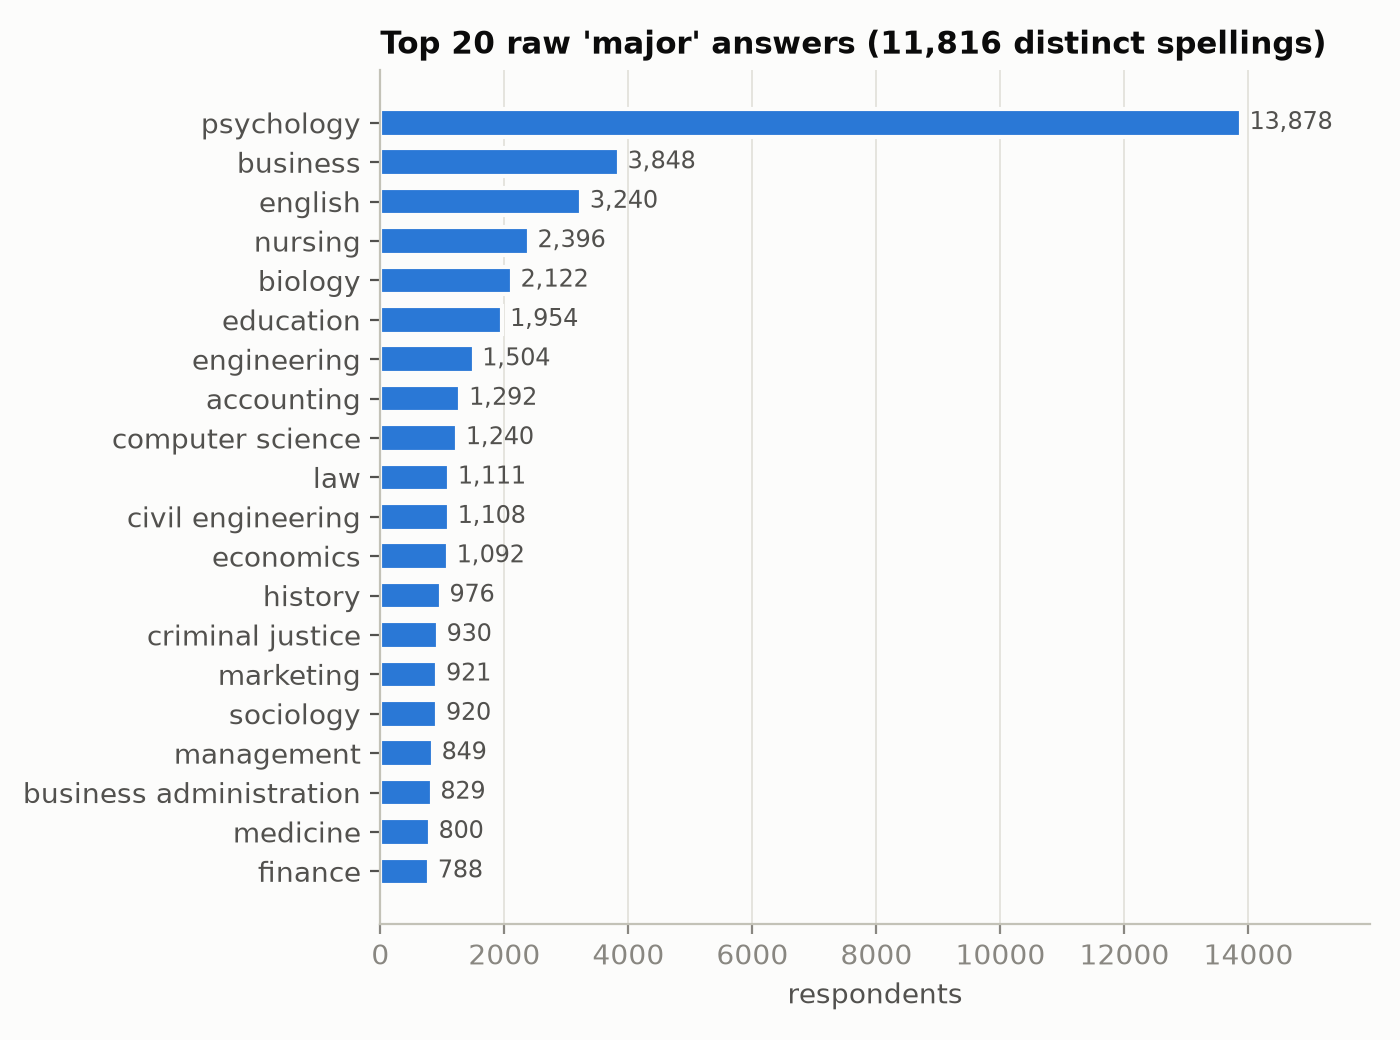
\includegraphics[width=\linewidth]{raw_majors_top20.png}
\caption{Raw free-text majors before mapping.}\label{fig:majors}\end{subfigure}
\hfill
\begin{subfigure}{0.49\linewidth}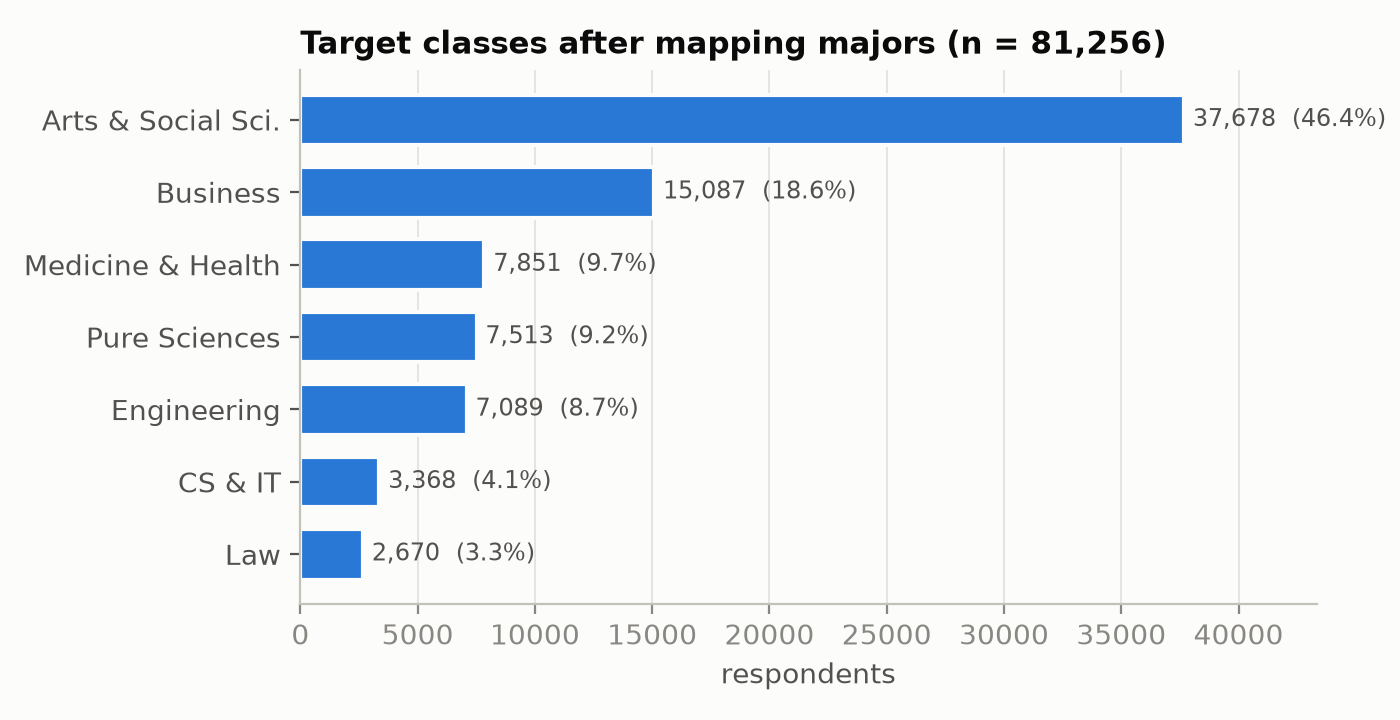
\includegraphics[width=\linewidth]{class_distribution.png}
\caption{Classes after mapping: 14:1 imbalance.}\label{fig:classes}\end{subfigure}
\caption{From 11,816 messy spellings to seven target classes.}
\end{figure}

\begin{figure}[H]
\centering
\begin{subfigure}{0.49\linewidth}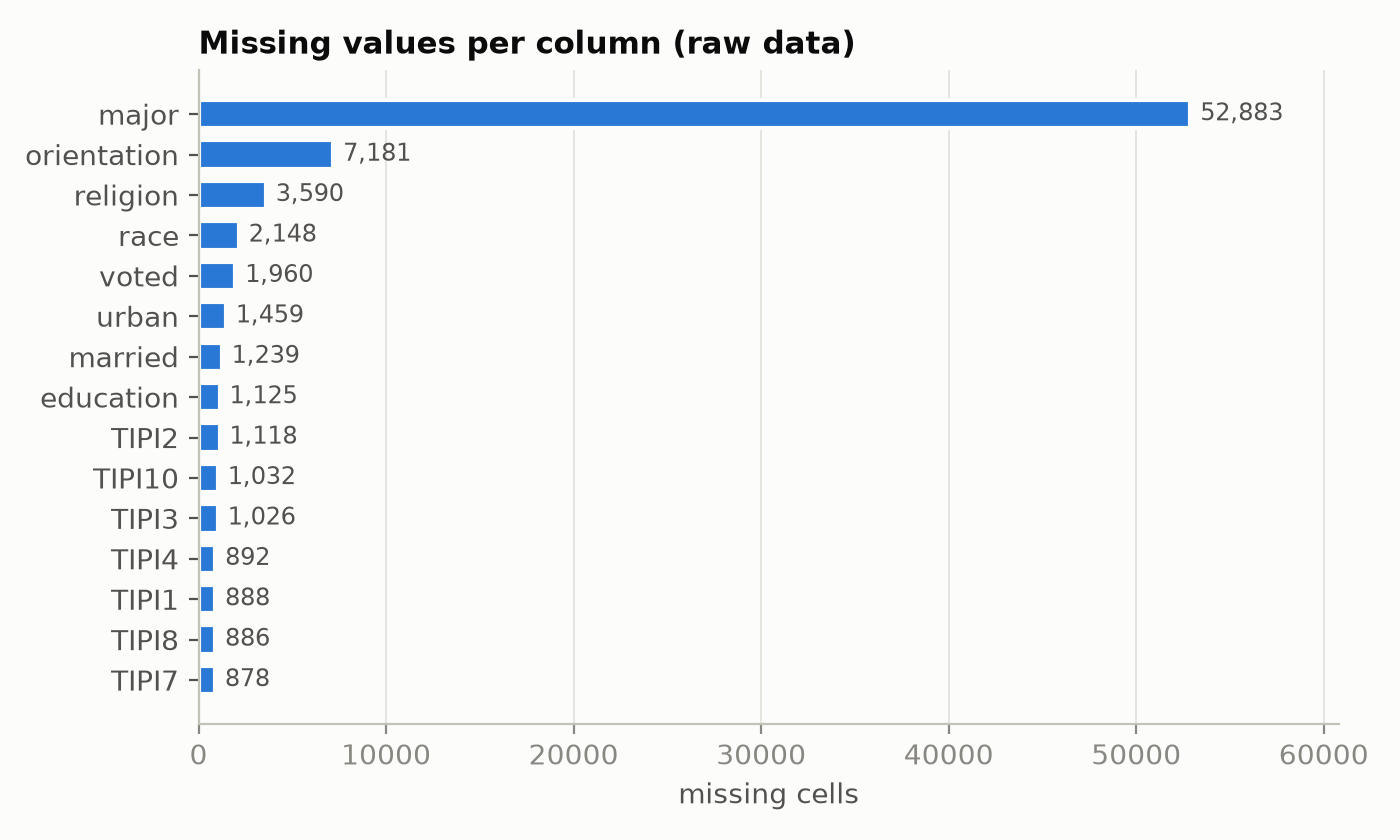
\includegraphics[width=\linewidth]{missing_values.png}
\caption{Missing values per column (raw).}\label{fig:missing}\end{subfigure}
\hfill
\begin{subfigure}{0.49\linewidth}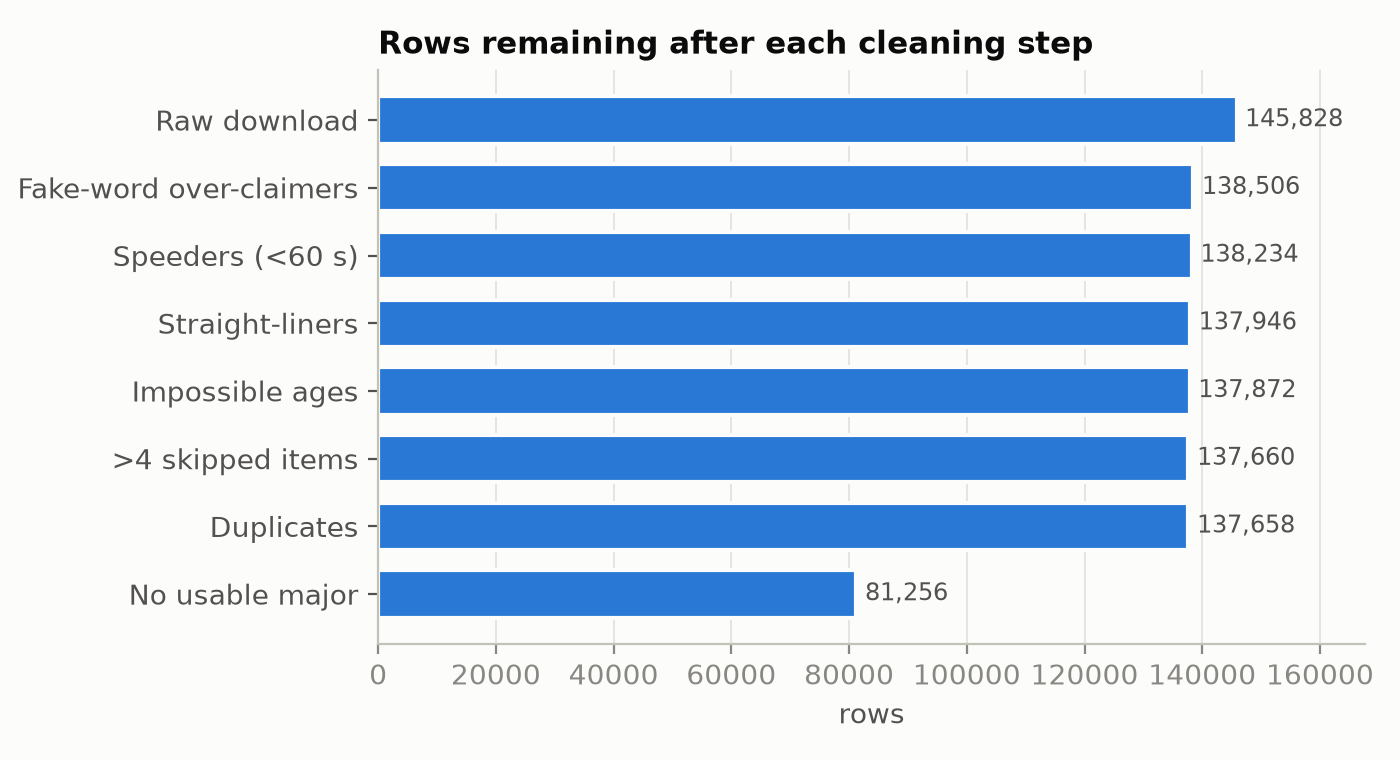
\includegraphics[width=\linewidth]{cleaning_funnel.png}
\caption{Rows remaining after each step.}\label{fig:funnel}\end{subfigure}
\caption{Data quality before cleaning. Most missing majors are blank answers. Orientation,
religion and race are missing more often but are not used.}
\end{figure}

\begin{figure}[H]
\centering
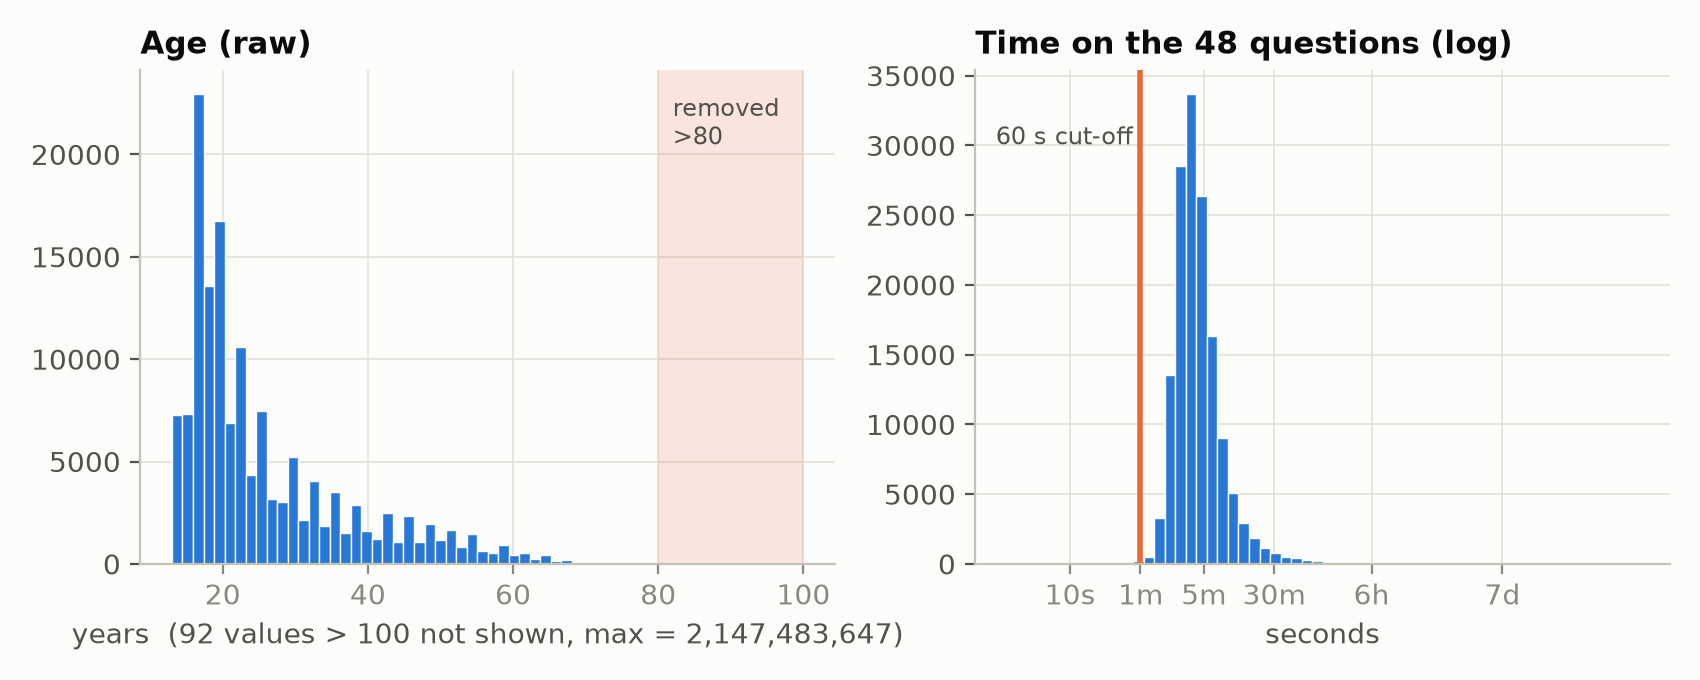
\includegraphics[width=0.85\linewidth]{outliers.png}
\caption{Outliers. Left: ages above 80 (and 92 values above 100, up to $2^{31}-1$) are removed.
Right: time spent on the test. Answers under 60\,s (orange line) are treated as speeders.}
\label{fig:outliers}
\end{figure}

\begin{figure}[H]
\centering
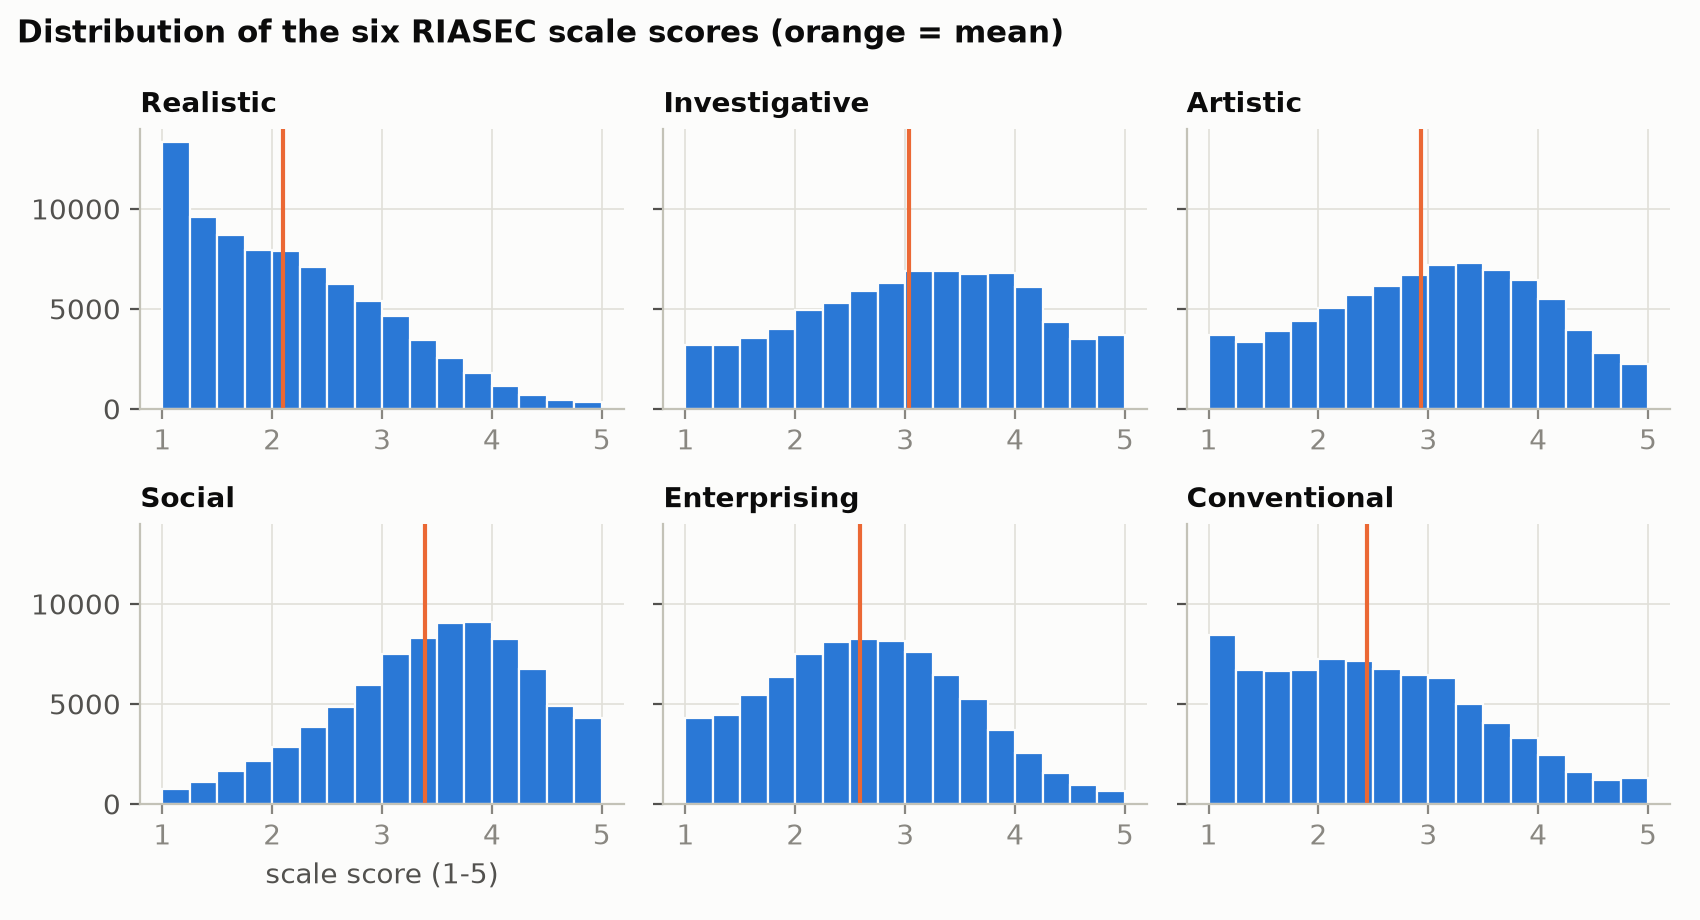
\includegraphics[width=0.85\linewidth]{riasec_distributions.png}
\caption{The six RIASEC scale scores. Social and Investigative lean high and Realistic and
Conventional lean low. This reflects the sample (two thirds women, many psychology majors), not
the population, which is one more reason for class weighting.}
\label{fig:dists}
\end{figure}

\begin{figure}[H]
\centering
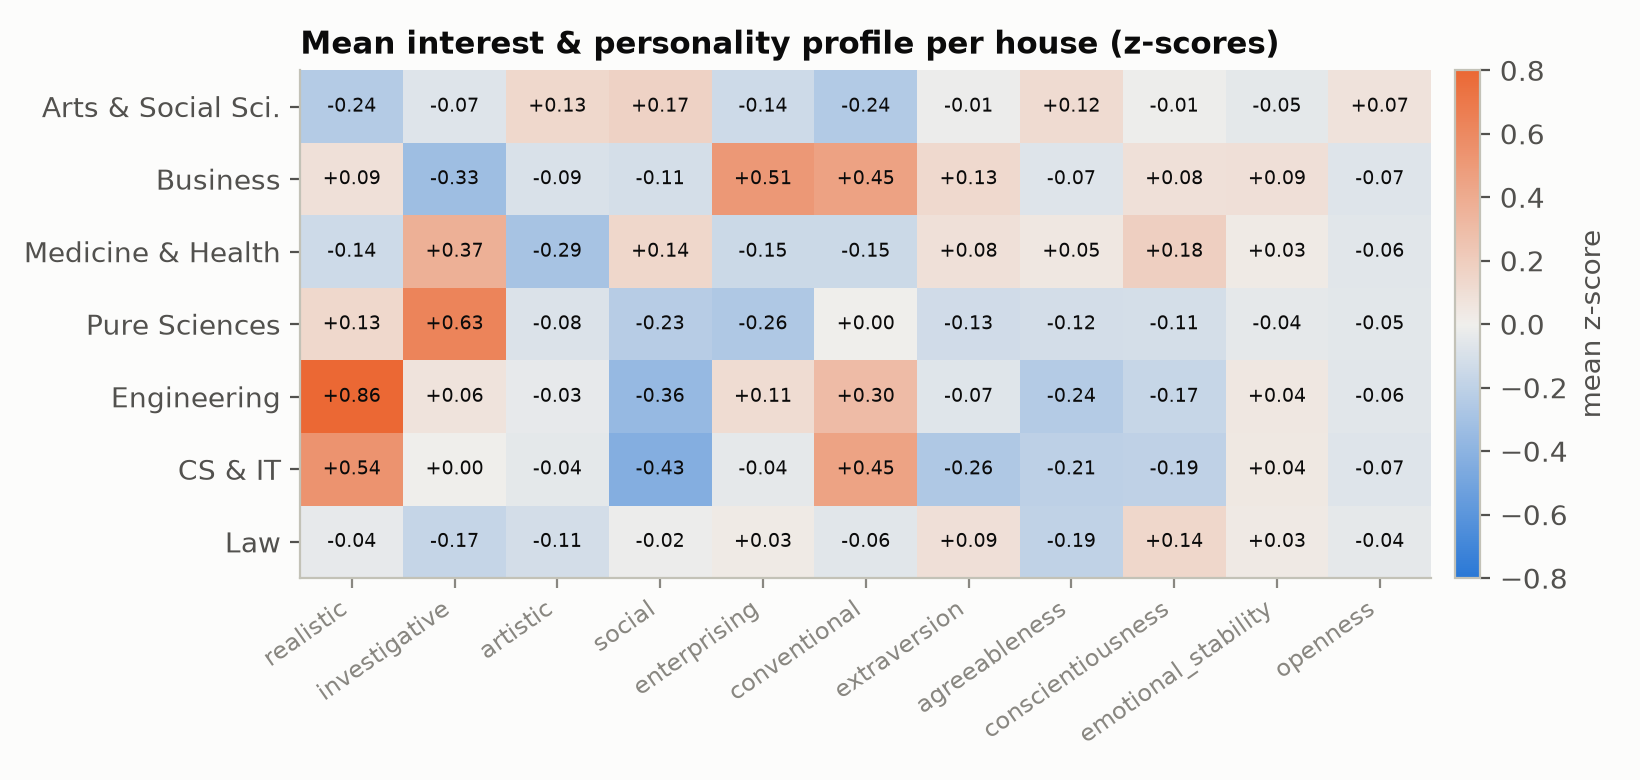
\includegraphics[width=0.95\linewidth]{house_profiles.png}
\caption{Mean profile of each house in z-scores. The data reproduces Holland's theory. Engineering
and CS are highest on Realistic, Medicine and Pure Sciences on Investigative, Business and Law on
Enterprising, and Arts \& Social Sciences on Social. The overlaps between pairs of houses are why
a single-rule system is not enough.}
\label{fig:profiles}
\end{figure}

\begin{figure}[H]
\centering
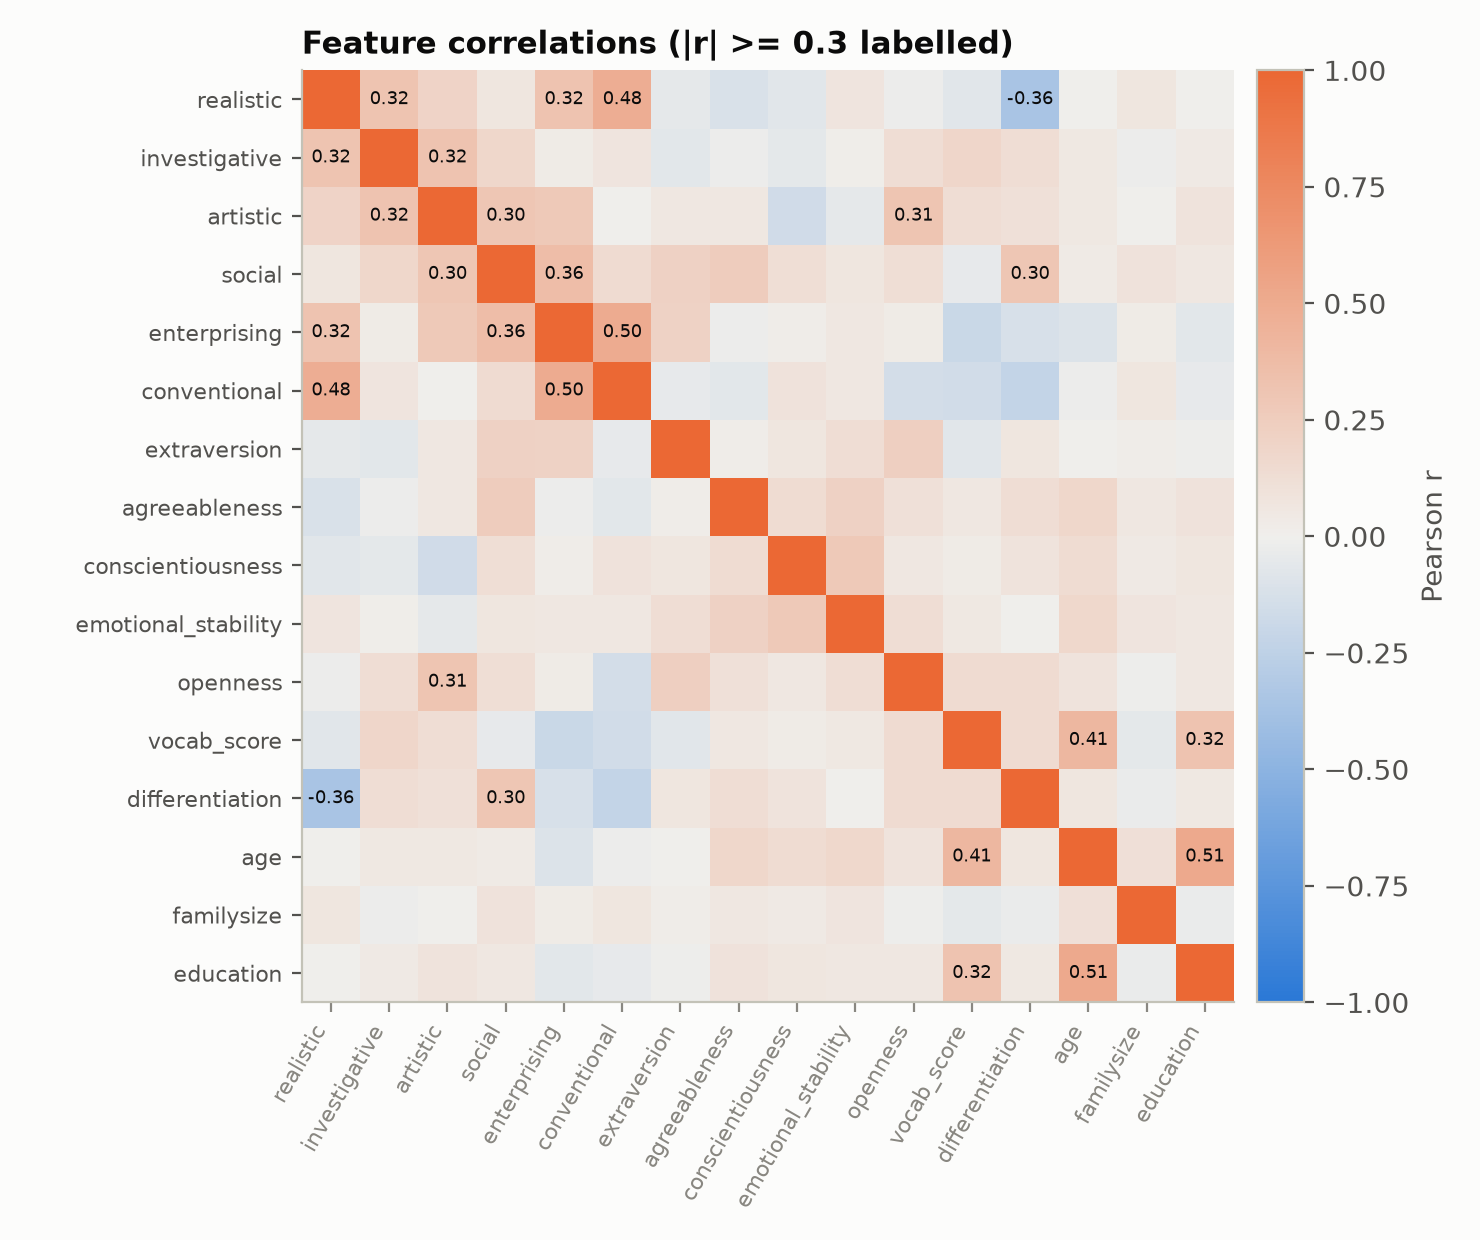
\includegraphics[width=0.7\linewidth]{feature_correlation.png}
\caption{Feature correlations. The strongest pairs are age--education ($r=0.51$),
Enterprising--Conventional (0.50) and Realistic--Conventional (0.48), matching the adjacency of
these types on Holland's hexagon. No pair is high enough ($|r|>0.8$) to require removing a
feature.}
\label{fig:corr}
\end{figure}

\begin{figure}[H]
\centering
\begin{subfigure}{0.52\linewidth}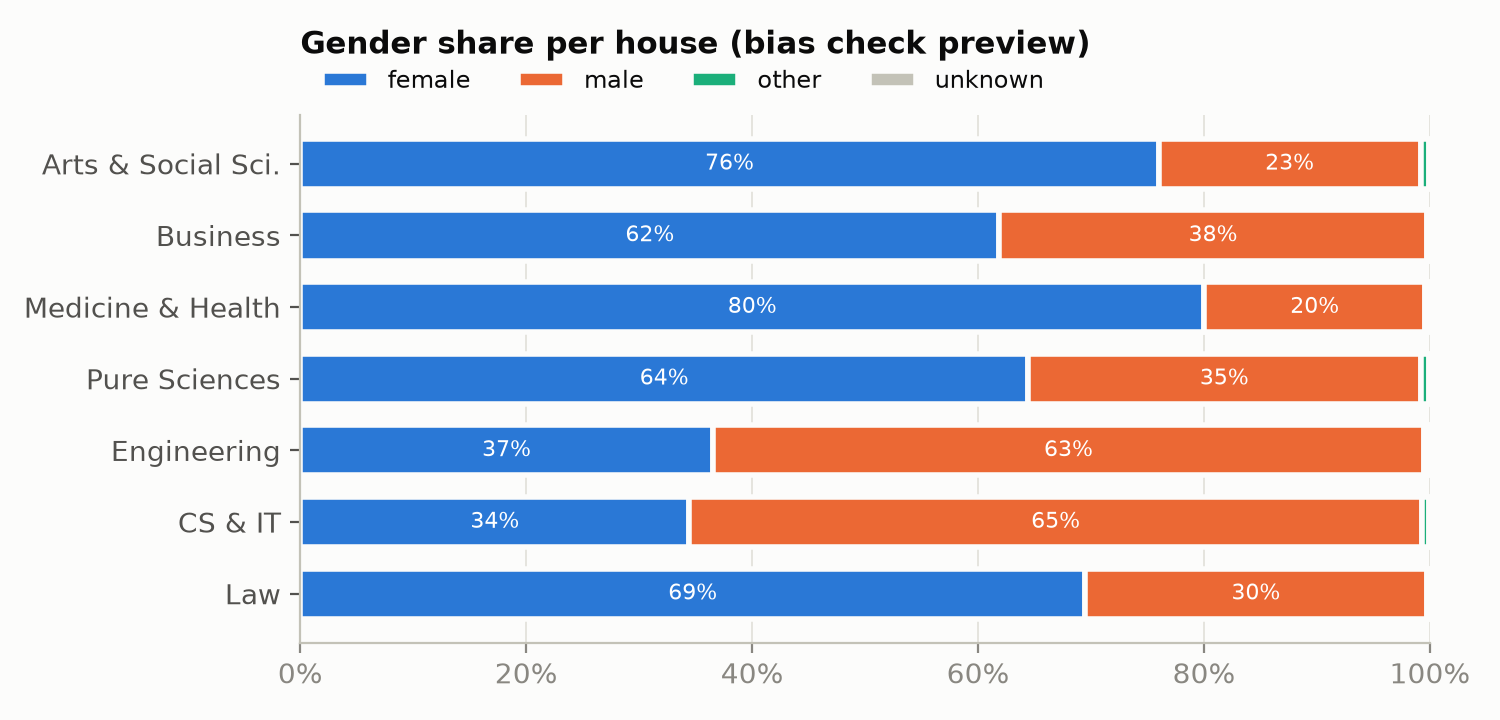
\includegraphics[width=\linewidth]{gender_by_house.png}
\caption{Gender share per house.}\label{fig:gender}\end{subfigure}
\hfill
\begin{subfigure}{0.46\linewidth}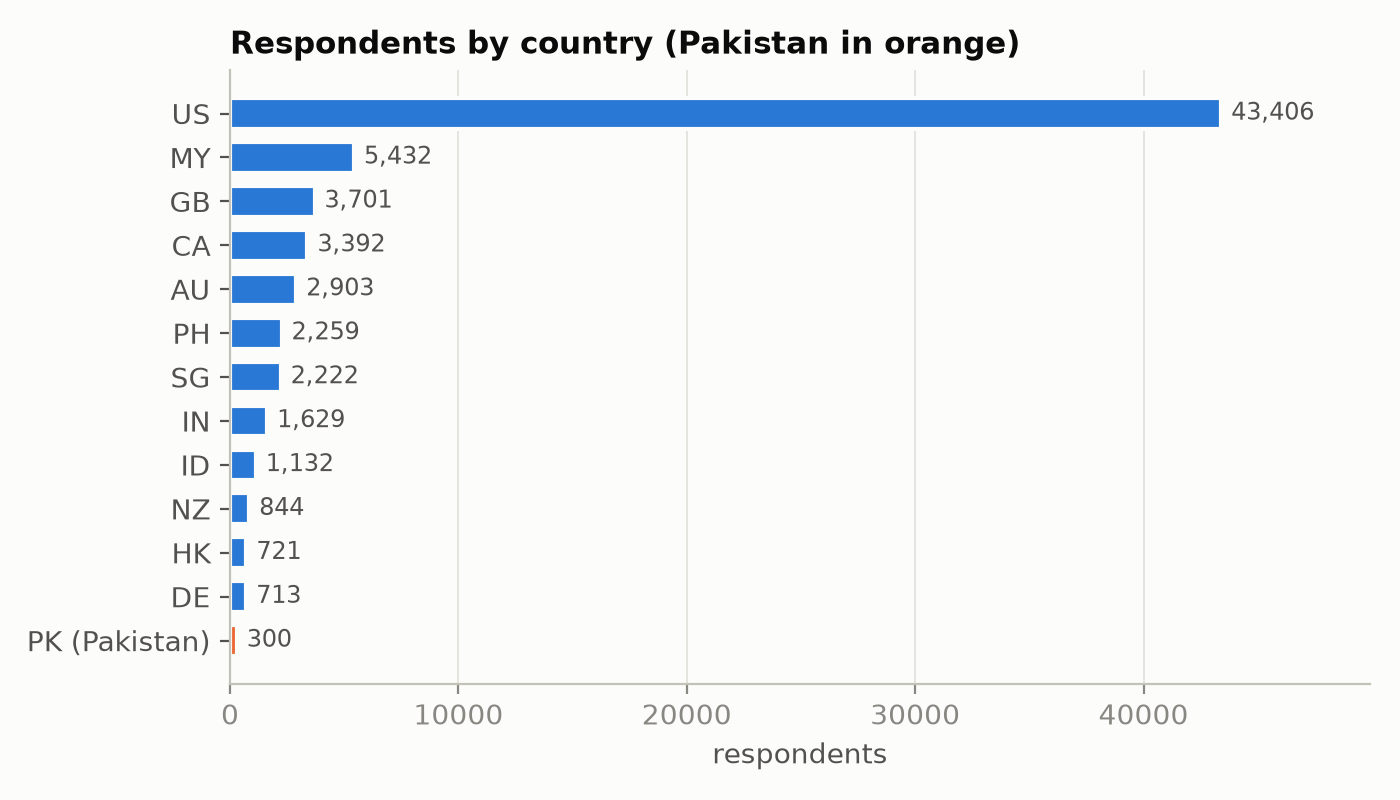
\includegraphics[width=\linewidth]{countries.png}
\caption{Country of respondents.}\label{fig:countries}\end{subfigure}
\caption{Two sources of bias to address in Phase~4. (a) Engineering and CS are about two-thirds
male, so a model could learn to recommend them less to women. Gender is therefore excluded from
the inputs and per-gender metrics will be reported. (b) 53\% of respondents are from the US and
only 300 are from Pakistan, a domain shift our own survey is designed to measure.}
\end{figure}

\subsection{Pakistan statistics}\label{sec:eda-pk}

\begin{figure}[H]
\centering
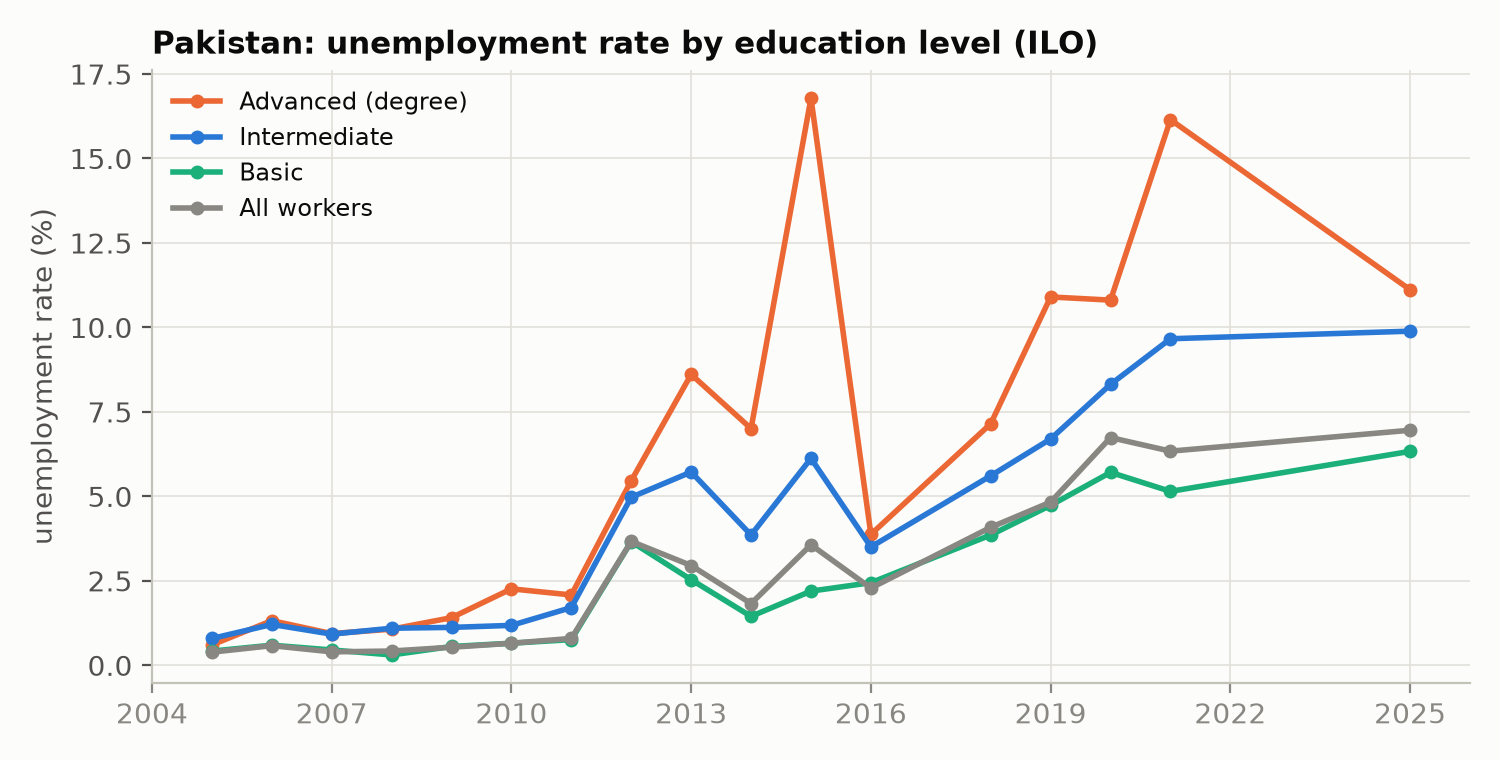
\includegraphics[width=0.8\linewidth]{pk_unemployment_by_education.png}
\caption{Unemployment rate by education level in Pakistan (ILOSTAT, Labour Force Survey). Since
2012, people with a degree have consistently had \emph{higher} unemployment than the workforce as
a whole, reaching 11.1\% in 2025. The jumps in 2015 and 2016 coincide with changes in survey
rounds and should be read with care.}
\label{fig:unemp}
\end{figure}

\begin{figure}[H]
\centering
\begin{subfigure}{0.5\linewidth}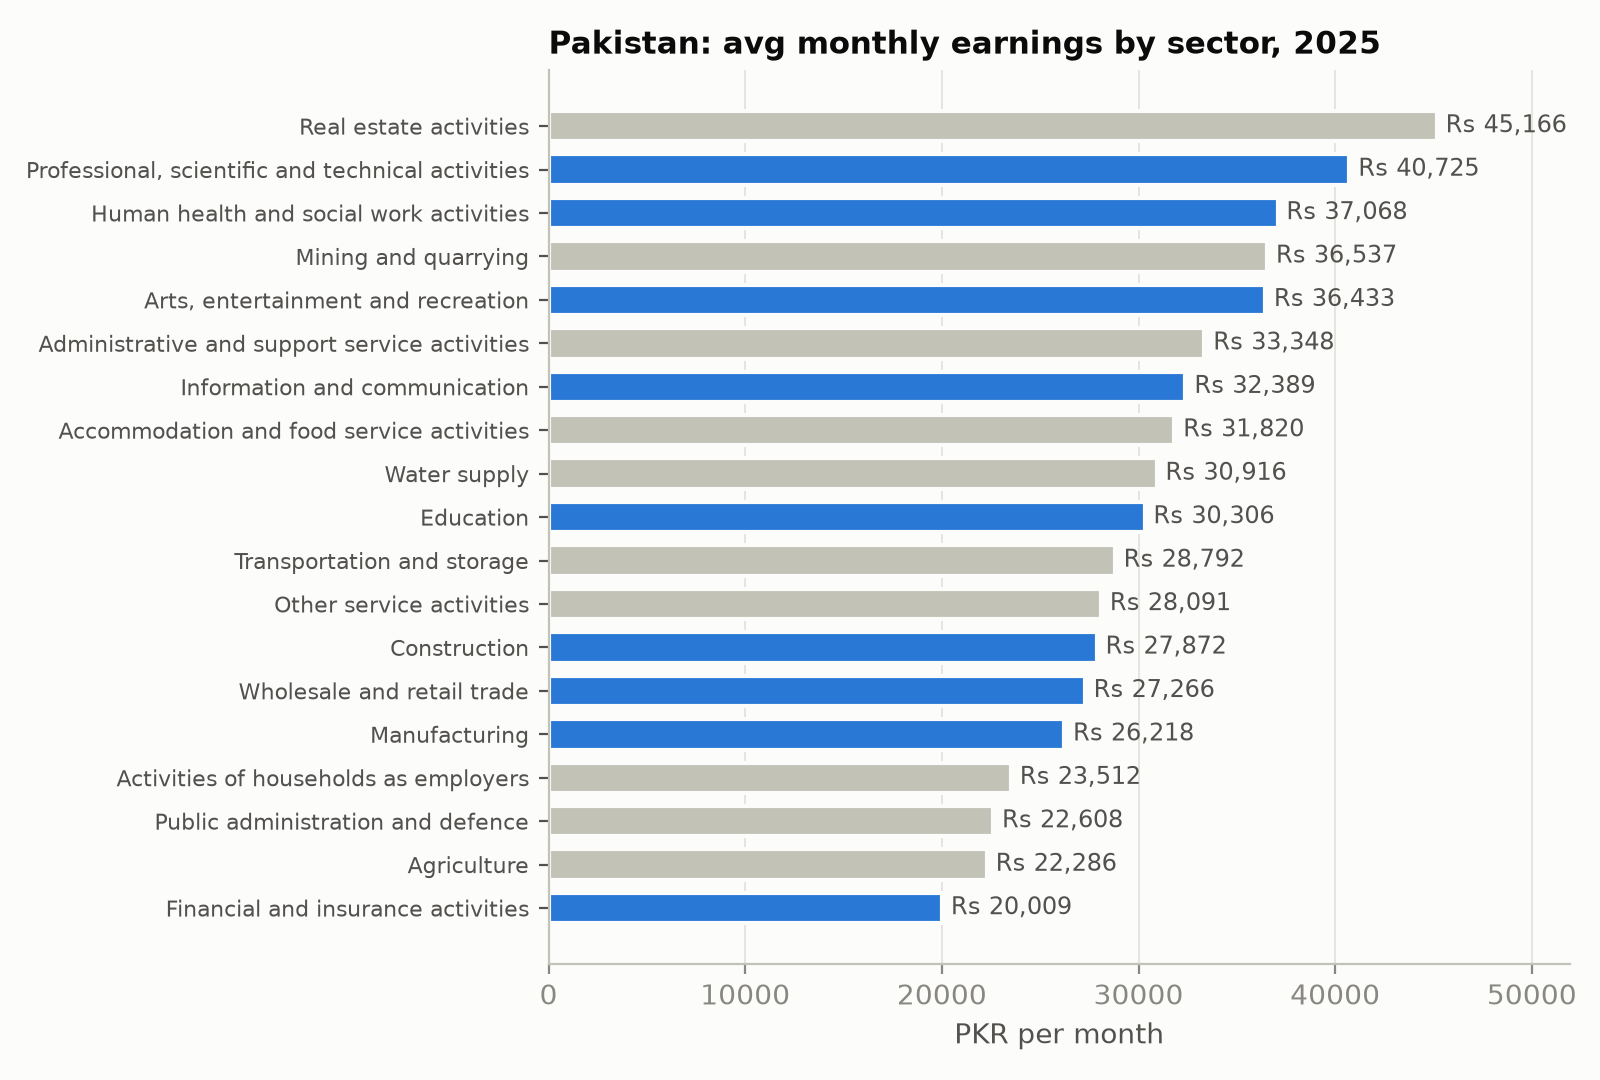
\includegraphics[width=\linewidth]{pk_sector_earnings.png}
\caption{Average monthly earnings by sector, 2025.}\label{fig:earn}\end{subfigure}
\hfill
\begin{subfigure}{0.48\linewidth}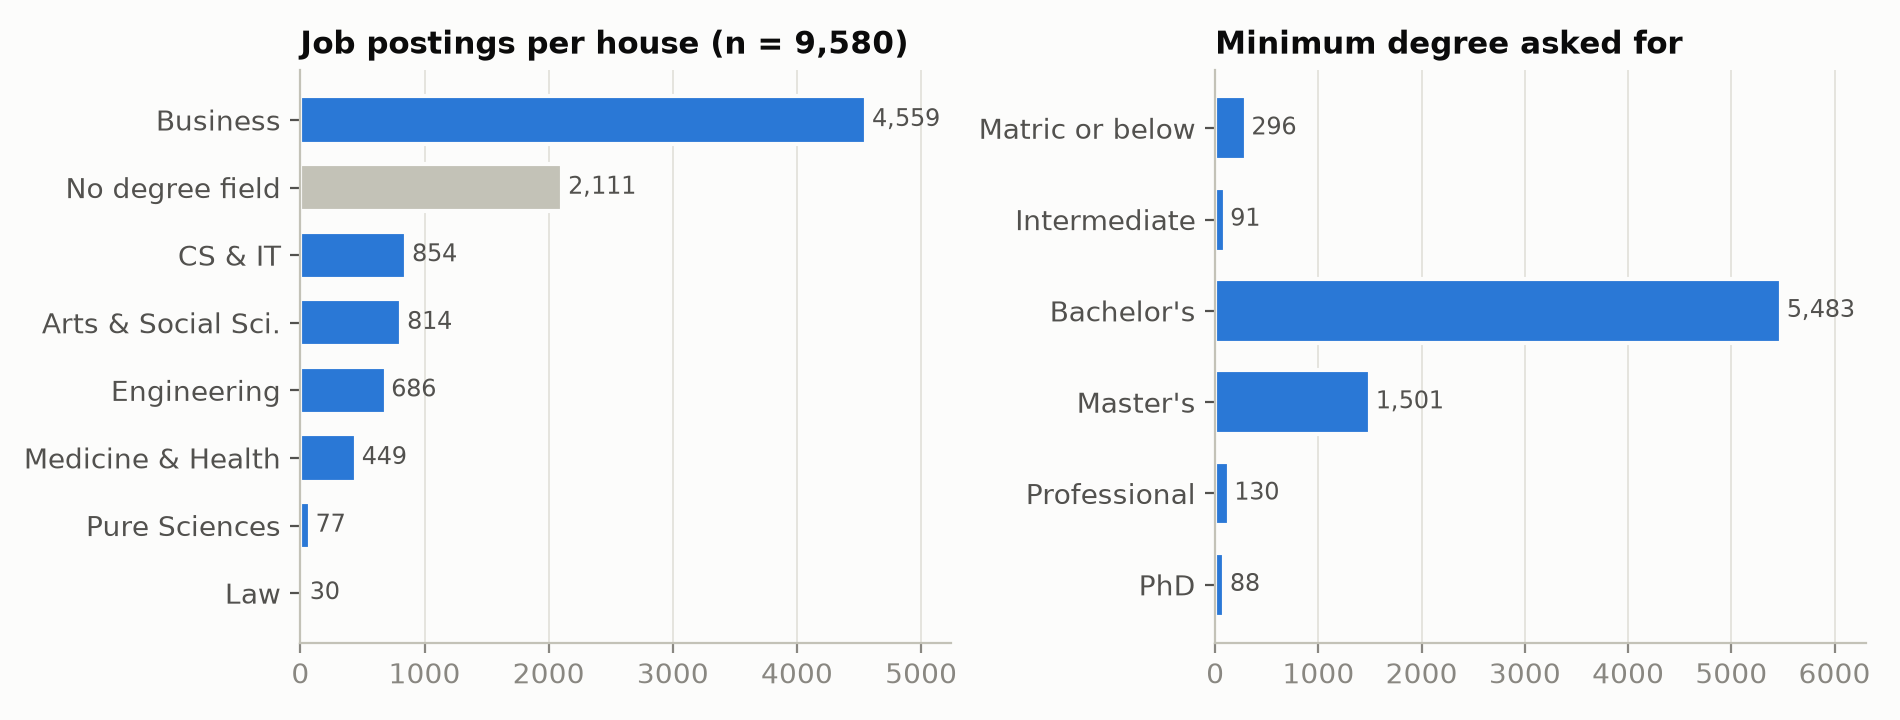
\includegraphics[width=\linewidth]{rozee_postings.png}
\caption{Rozee.pk postings by house and degree asked for.}\label{fig:rozee}\end{subfigure}
\caption{(a) Sector averages include all employees in a sector (a hospital's cleaners as well as
its doctors), so they are a coarse proxy for a degree's value. The low figure for finance in
particular needs checking against occupation-level data in Phase~3. (b) Business roles dominate
current postings (sales and marketing), and 72\% of postings that state a degree ask for a
bachelor's.}
\end{figure}

% ------------------------------------------------------------------
\section{Preliminary Baseline (preview of Phase 3)}
To check that the prepared data supports the task, we trained quick baselines on the split
from Section~4 (\texttt{baseline\_models.py}). Because the app will show every student a ranked
list of houses, we report top-$k$ accuracy (is the true house among the $k$ most probable?) next
to ordinary accuracy and macro-F1.

\begin{table}[H]
\centering\small
\caption{Baselines on the held-out test set (16,252 students, 7 houses).}
\label{tab:baseline}
\begin{tabular}{@{}lrrrr@{}}
\toprule
Model & Top-1 & Top-2 & Top-3 & Macro-F1 \\
\midrule
Always predict the largest house & 46.4\% & -- & -- & -- \\
Logistic regression, class-balanced & 36.8\% & 55.1\% & 71.4\% & 0.30 \\
Gradient boosting, 30 features & 53.0\% & 73.0\% & 83.4\% & 0.28 \\
\textbf{Gradient boosting, 30 features + 58 raw answers} & \textbf{56.6\%} & \textbf{76.2\%} & \textbf{86.0\%} & \textbf{0.35} \\
\bottomrule
\end{tabular}
\end{table}

\begin{itemize}
\item \textbf{Top-1 accuracy alone is misleading.} Always predicting Arts \& Social Sciences already
      scores 46.4\%. Class balancing lowers top-1 accuracy (36.8\%) but raises macro-F1, because
      the model stops ignoring Law and CS.
\item \textbf{Interests predict a field only moderately.} People with the same interest profile
      study different subjects, so a single-answer accuracy of 70--80\% is not realistic from this
      data. Restricting training to graduates did not change the result. The best model's top-3
      list contains the student's actual field \textbf{86\%} of the time, which supports
      presenting the top three houses with probabilities rather than a single verdict.
\item \textbf{Where further gains must come from:} new signals rather than more of the same
      data. These are the task-based career simulations planned for the app, the Pakistani
      survey, and tuning of the gradient-boosting and neural models in Phase~3.
\end{itemize}

% ------------------------------------------------------------------
\section{Challenges and Limitations}
\begin{itemize}
\item \textbf{Label noise.} Majors are self-reported free text, and some respondents are students
      who may still switch. The keyword mapping is transparent and testable, but imperfect.
\item \textbf{Domain shift.} The training data is mostly from the US and the users are Pakistani.
      Only 300 Pakistani rows exist. Our survey is the planned fix, but it has no responses yet.
\item \textbf{Proxy statistics.} No public dataset gives earnings per \emph{degree} in Pakistan,
      so sector-level ILO data and job postings stand in for it. PBS microdata, which must be
      requested, would allow degree-level figures.
\item \textbf{Salaries on Rozee.pk} are hidden behind a login for most postings, so salary comes
      only from ILO data.
\end{itemize}

\section{Next Steps (Phases 3--4)}
Train and compare logistic regression, random forest, gradient boosting and an MLP on the
prepared split with class weights. Report accuracy, macro-F1 and a confusion matrix. Run the bias
check by gender and on the Pakistani subset. Build the hosted web app and report generator.

\section*{Repository}
\begin{tabular}{@{}ll@{}}
\texttt{data\_scripts/collect\_data.py} & downloads all raw sources, writes the collection log \\
\texttt{data\_scripts/house\_mapping.py} & free text $\rightarrow$ house rules \\
\texttt{data\_scripts/clean\_riasec.py} & missing values, validity, outliers, duplicates, labels \\
\texttt{data\_scripts/clean\_pakistan.py} & ILO, World Bank and Rozee.pk cleaning \\
\texttt{data\_scripts/build\_features.py} & feature engineering, scaling, encoding, split \\
\texttt{data\_scripts/eda.py} & all figures in this report \\
\texttt{data\_scripts/evaluate\_supplementary.py} & learnability test of the Kaggle datasets (Table~\ref{tab:excluded}) \\
\texttt{data\_scripts/baseline\_models.py} & preliminary baselines (Table~\ref{tab:baseline}) \\
\end{tabular}

\begin{thebibliography}{9}\small
\bibitem{holland} J.~L.~Holland, \emph{Making Vocational Choices: A Theory of Vocational Personalities and Work Environments}, 3rd ed. Psychological Assessment Resources, 1997.
\bibitem{tipi} S.~D.~Gosling, P.~J.~Rentfrow and W.~B.~Swann, ``A very brief measure of the Big-Five personality domains,'' \emph{Journal of Research in Personality}, 37, 504--528, 2003.
\bibitem{op} Open Psychometrics, RIASEC raw data (collected 2015--2018), \url{http://openpsychometrics.org/_rawdata/}.
\bibitem{onet} National Center for O*NET Development, O*NET 31.0 Database, \url{https://www.onetcenter.org/database.html} (CC BY 4.0).
\bibitem{ilo} International Labour Organization, ILOSTAT SDMX API, \url{https://sdmx.ilo.org}.
\bibitem{wb} World Bank, World Development Indicators API, \url{https://api.worldbank.org}.
\bibitem{rozee} Rozee.pk job search, \url{https://www.rozee.pk}, accessed 18 October 2026.
\end{thebibliography}

\end{document}
